%%%%%%%%%%%%%%%%%%%%%%%%%%%%%%%%%%%%%%%%%
% Arsclassica Article
% LaTeX Template
% Version 1.1 (1/8/17)
%
% This template has been downloaded from:
% http://www.LaTeXTemplates.com
%
% Original author:
% Lorenzo Pantieri (http://www.lorenzopantieri.net) with extensive modifications by:
% Vel (vel@latextemplates.com)
%
% License:
% CC BY-NC-SA 3.0 (http://creativecommons.org/licenses/by-nc-sa/3.0/)
%
%%%%%%%%%%%%%%%%%%%%%%%%%%%%%%%%%%%%%%%%%

%----------------------------------------------------------------------------------------
%	PACKAGES AND OTHER DOCUMENT CONFIGURATIONS
%----------------------------------------------------------------------------------------

\documentclass[
18pt, % Main document font size
a4paper, % Paper type, use 'letterpaper' for US Letter paper
oneside, % One page layout (no page indentation)
%twoside, % Two page layout (page indentation for binding and different headers)
headinclude,footinclude, % Extra spacing for the header and footer
%BCOR5mm, % Binding correction
]{scrartcl}

%%%%%%%%%%%%%%%%%%%%%%%%%%%%%%%%%%%%%%%%%
% Arsclassica Article
% Structure Specification File
%
% This file has been downloaded from:
% http://www.LaTeXTemplates.com
%
% Original author:
% Lorenzo Pantieri (http://www.lorenzopantieri.net) with extensive modifications by:
% Vel (vel@latextemplates.com)
%
% License:
% CC BY-NC-SA 3.0 (http://creativecommons.org/licenses/by-nc-sa/3.0/)
%
%%%%%%%%%%%%%%%%%%%%%%%%%%%%%%%%%%%%%%%%%

%----------------------------------------------------------------------------------------
%	REQUIRED PACKAGES
%----------------------------------------------------------------------------------------

\usepackage[
nochapters, % Turn off chapters since this is an article        
beramono, % Use the Bera Mono font for monospaced text (\texttt)
eulermath,% Use the Euler font for mathematics
pdfspacing, % Makes use of pdftex’ letter spacing capabilities via the microtype package
dottedtoc % Dotted lines leading to the page numbers in the table of contents
]{classicthesis} % The layout is based on the Classic Thesis style

\usepackage{arsclassica} % Modifies the Classic Thesis package

\usepackage{float}

\usepackage[T1]{fontenc} % Use 8-bit encoding that has 256 glyphs

\usepackage[utf8]{inputenc} % Required for including letters with accents

\usepackage{graphicx} % Required for including images
\graphicspath{{Figures/}} % Set the default folder for images

\usepackage{enumitem} % Required for manipulating the whitespace between and within lists

\usepackage{lipsum} % Used for inserting dummy 'Lorem ipsum' text into the template

\usepackage{subfig} % Required for creating figures with multiple parts (subfigures)

\usepackage{amsmath,amssymb,amsthm} % For including math equations, theorems, symbols, etc

\usepackage{varioref} % More descriptive referencing

%----------------------------------------------------------------------------------------
%	THEOREM STYLES
%---------------------------------------------------------------------------------------

\theoremstyle{definition} % Define theorem styles here based on the definition style (used for definitions and examples)
\newtheorem{definition}{Definition}

\theoremstyle{plain} % Define theorem styles here based on the plain style (used for theorems, lemmas, propositions)
\newtheorem{theorem}{Theorem}

\theoremstyle{remark} % Define theorem styles here based on the remark style (used for remarks and notes)

%----------------------------------------------------------------------------------------
%	HYPERLINKS
%---------------------------------------------------------------------------------------

\hypersetup{
%draft, % Uncomment to remove all links (useful for printing in black and white)
colorlinks=true, breaklinks=true, bookmarks=true,bookmarksnumbered,
urlcolor=webbrown, linkcolor=RoyalBlue, citecolor=webgreen, % Link colors
pdftitle={}, % PDF title
pdfauthor={\textcopyright}, % PDF Author
pdfsubject={}, % PDF Subject
pdfkeywords={}, % PDF Keywords
pdfcreator={pdfLaTeX}, % PDF Creator
pdfproducer={LaTeX with hyperref and ClassicThesis} % PDF producer
} % Include the structure.tex file which specified the document structure and layout

\hyphenation{Fortran hy-phen-ation} % Specify custom hyphenation points in words with dashes where you would like hyphenation to occur, or alternatively, don't put any dashes in a word to stop hyphenation altogether
\usepackage{stix} % Use the STIX fonts

%----------------------------------------------------------------------------------------
%	TITLE AND AUTHOR(S)
%----------------------------------------------------------------------------------------

\title{\normalfont\spacedallcaps{Op}} % The article title

%\subtitle{Subtitle} % Uncomment to display a subtitle

\date{} % An optional date to appear under the author(s)

%----------------------------------------------------------------------------------------

\begin{document}

%----------------------------------------------------------------------------------------
%	HEADERS
%----------------------------------------------------------------------------------------

\renewcommand{\sectionmark}[1]{\markright{\spacedlowsmallcaps{#1}}} % The header for all pages (oneside) or for even pages (twoside)
%\renewcommand{\subsectionmark}[1]{\markright{\thesubsection~#1}} % Uncomment when using the twoside option - this modifies the header on odd pages
\lehead{\mbox{\llap{\small\thepage\kern1em\color{halfgray} \vline}\color{halfgray}\hspace{0.5em}\rightmark\hfil}} % The header style

\pagestyle{scrheadings} % Enable the headers specified in this block

%----------------------------------------------------------------------------------------
%	TABLE OF CONTENTS & LISTS OF FIGURES AND TABLES
%----------------------------------------------------------------------------------------

%\maketitle % Print the title/author/date block

\setcounter{tocdepth}{2} % Set the depth of the table of contents to show sections and subsections only

\tableofcontents % Print the table of contents


%----------------------------------------------------------------------------------------
%	AUTHOR AFFILIATIONS
%----------------------------------------------------------------------------------------

%\let\thefootnote\relax\footnotetext{* \textit{Research Head, Idaho Catfish Project, Coeur d'Alene, Idaho}}

%----------------------------------------------------------------------------------------

\newpage % Start the article content on the second page, remove this if you have a longer abstract that goes onto the second page

%----------------------------------------------------------------------------------------
%	INTRODUCTION
%----------------------------------------------------------------------------------------

\section{Introduction}
\subsection*{Overview}

Northern Idaho is one of the regions in the western United States that has seen extensive mining operations. The South fork of the Coeur d’Alene river has carried heavy metal contaminated sediments from silver and lead mining to the Coeur d’Alene lakebed. By developing an underwater drone capable of descending to deep-water, we become able to read the water quality in lakes and reservoirs. This will allow better supervision of water bodies and management of toxicity.

\subsection*{Purpose \& Scope}

This project focuses on creating and/or beginning development of an autonomous submarine that will collect water quality data in deep-water lakes and reservoirs. This submarine, dubbed the “Idaho Catfish”, will be able to perform such underwater surveys by continuously sampling a variety of water quality variables such as oxygen, pH, temperature, etc. The end result will be that the Catfish will be fully autonomous, but tethered instructions will also be provided.

\subsection*{The Submarine}
The submarine itself has been provided by Gizmo Coeur d'Alene and is a small sized submarine and handling gear set. The Catfish has been to the bottom of Lake Pend Oreille and is confirmed to be airtight and functional at 1200 feet under the water. It is speculated that it is good to go under up to 1600 feet but this is untested.

\subsection*{Term Definitions}

\textit{Ballast} - heavy material, such as gravel, sand, iron, or lead, placed low in a vessel to improve its stability. \\ \\
\textit{Handling Gear} - The set of gear that aids in deploying the submarine. Contains the tether, a winch, battery, communications module, and various storage. See Diagram \\ \\
\textit{Idaho Catfish }  – The submarine nickname. \\ \\
\textit{O-Ring} - a gasket in the form of a ring with a circular cross section, typically made of pliable material, used to seal connections in pipes, tubes, etc. \\ \\
\textit{Tethered } – The wires that connect the submarine to the surface, allowing for direct control and easier tracking of the submarine. Currently the submarine only runs tethered, it is not fully autonomous. \\ \\
\textit{ V } - Stands for voltage, a way of measuring a charge in batteries. \\ \\

\newpage
 
%----------------------------------------------------------------------------------------
%	BASIC OPS
%----------------------------------------------------------------------------------------

\section{Basic Operations}
\subsection{Components}
\vspace*{5mm}
\begin{figure}[H]
	\centering 
	\hspace*{-2.5cm}
	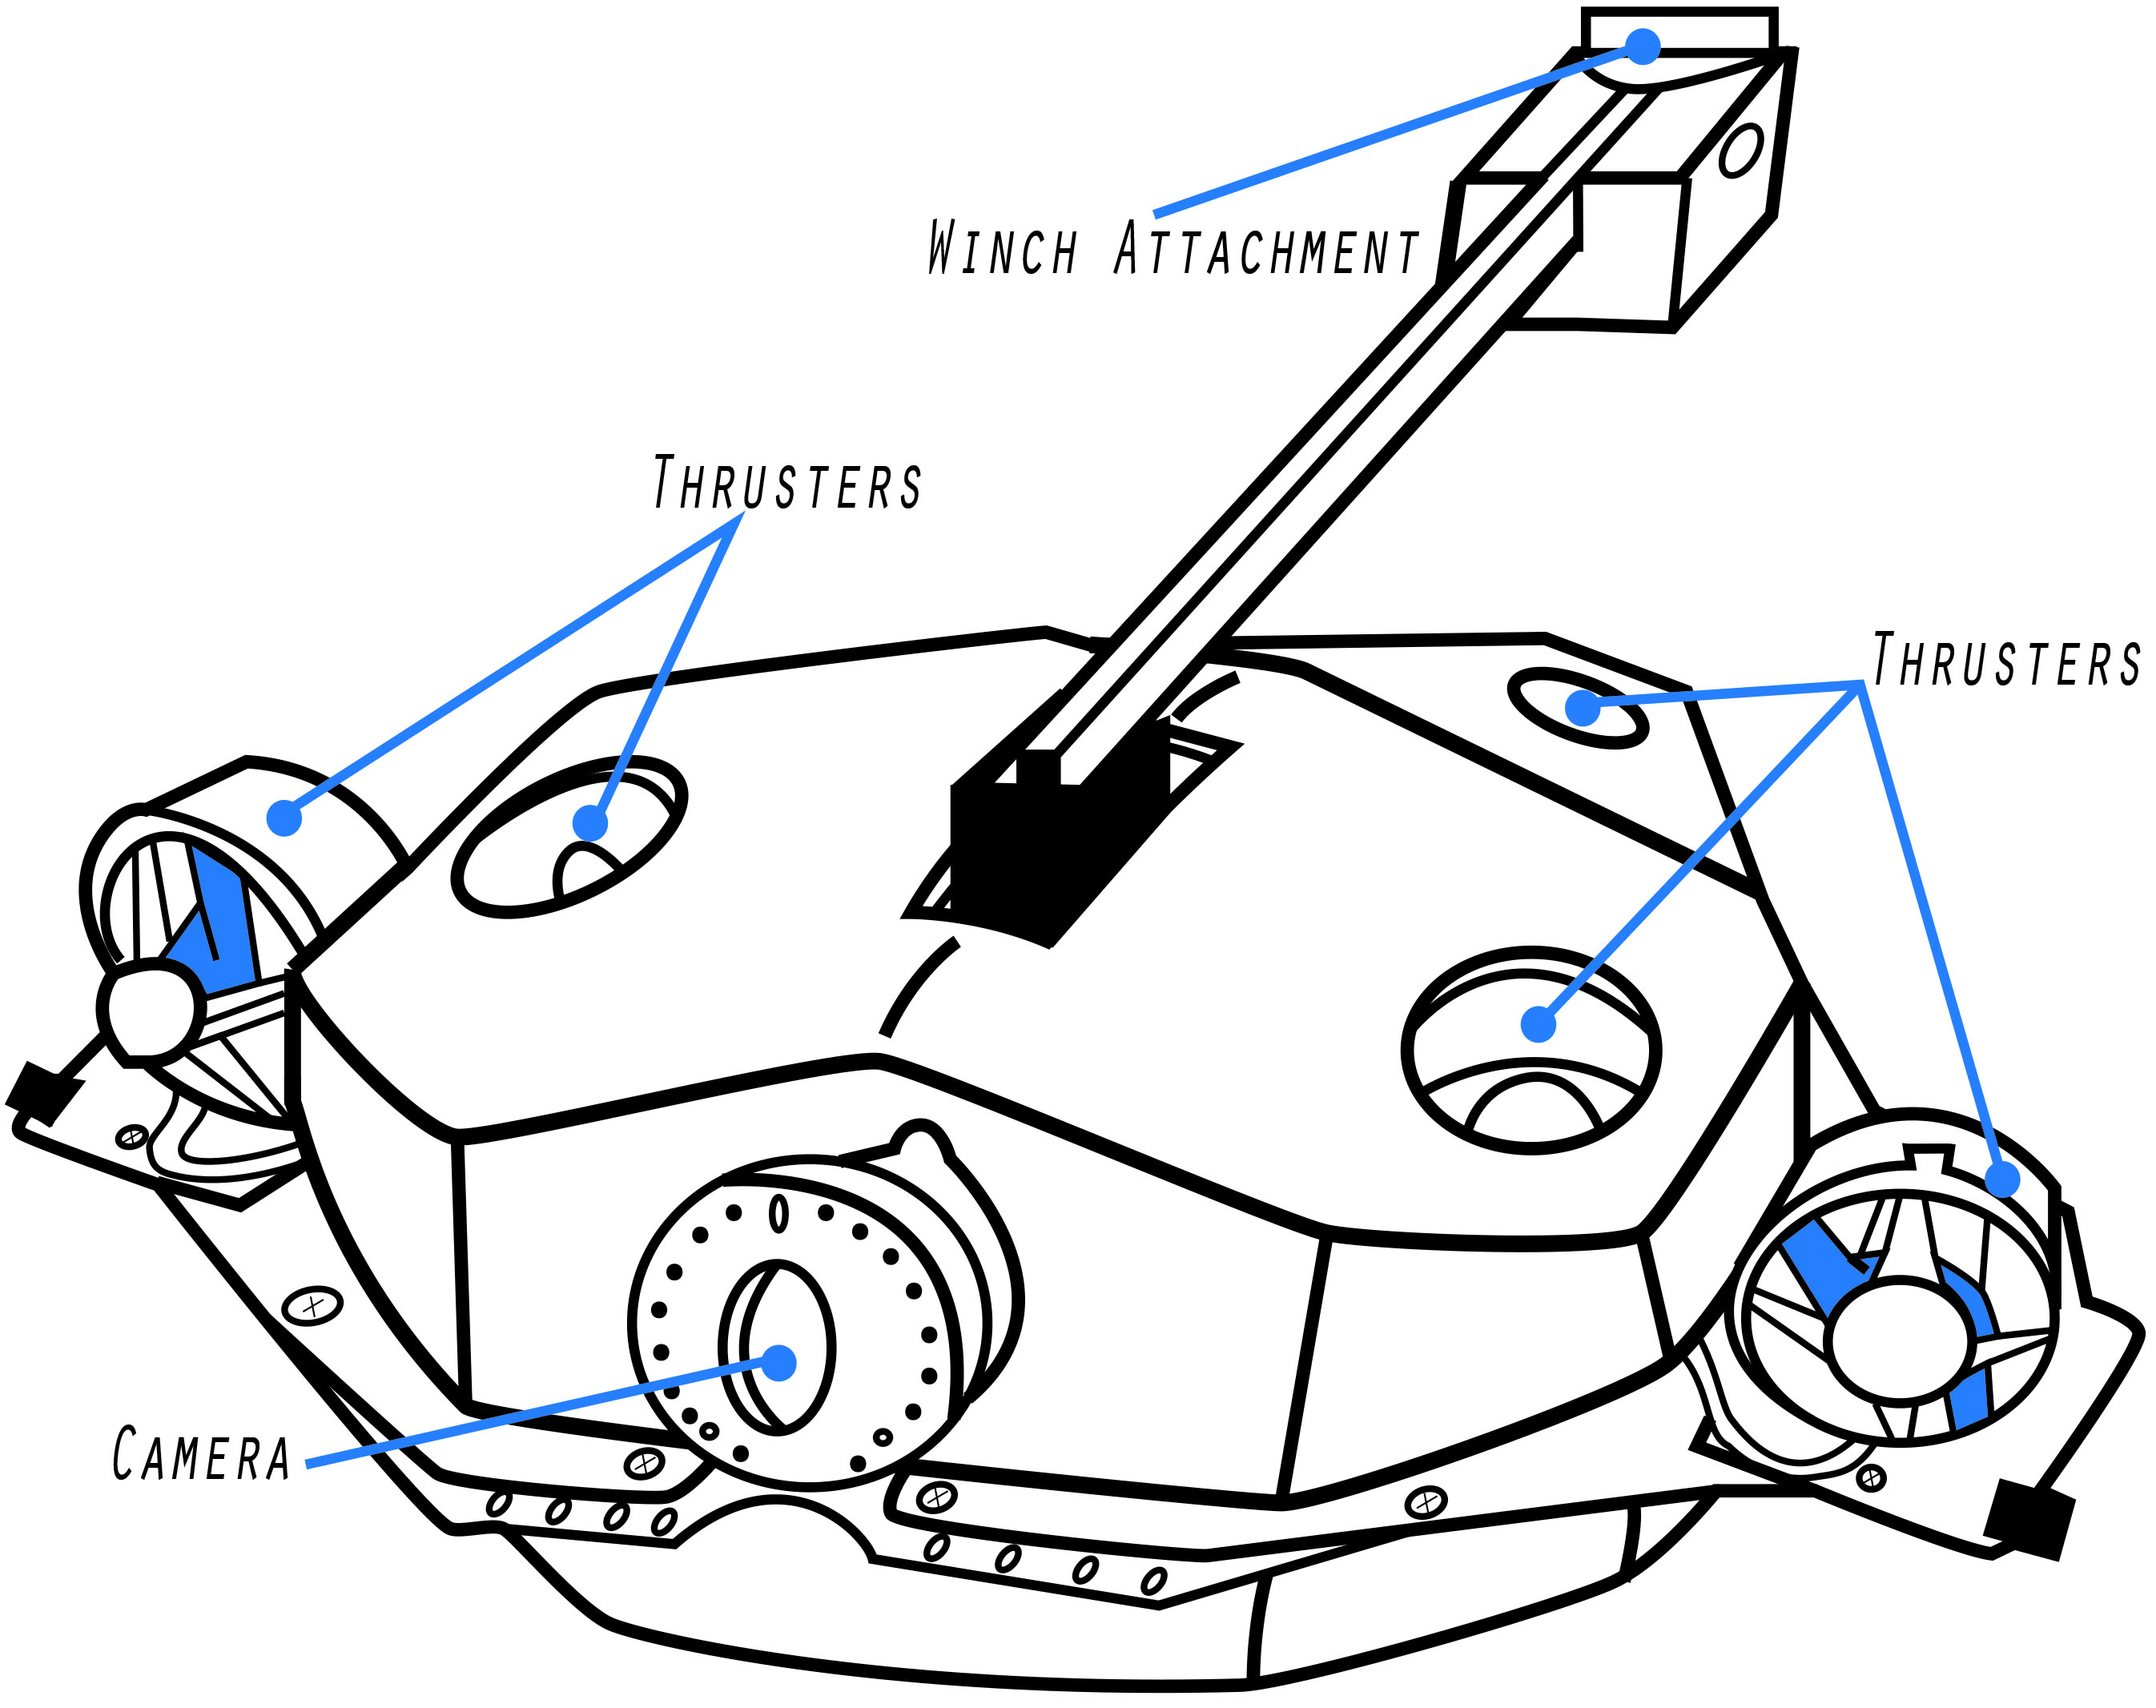
\includegraphics[width=1.4\linewidth]{Figures/Component_Diagrams/basic_sub.jpg}
	\caption[]{An overview of the submarine} % The text in the square bracket is the caption for the list of figures while the text in the curly brackets is the figure caption 
\end{figure}
\vspace*{5mm}
\begin{figure}[H]
	\centering 
	\hspace*{-2.5cm}
	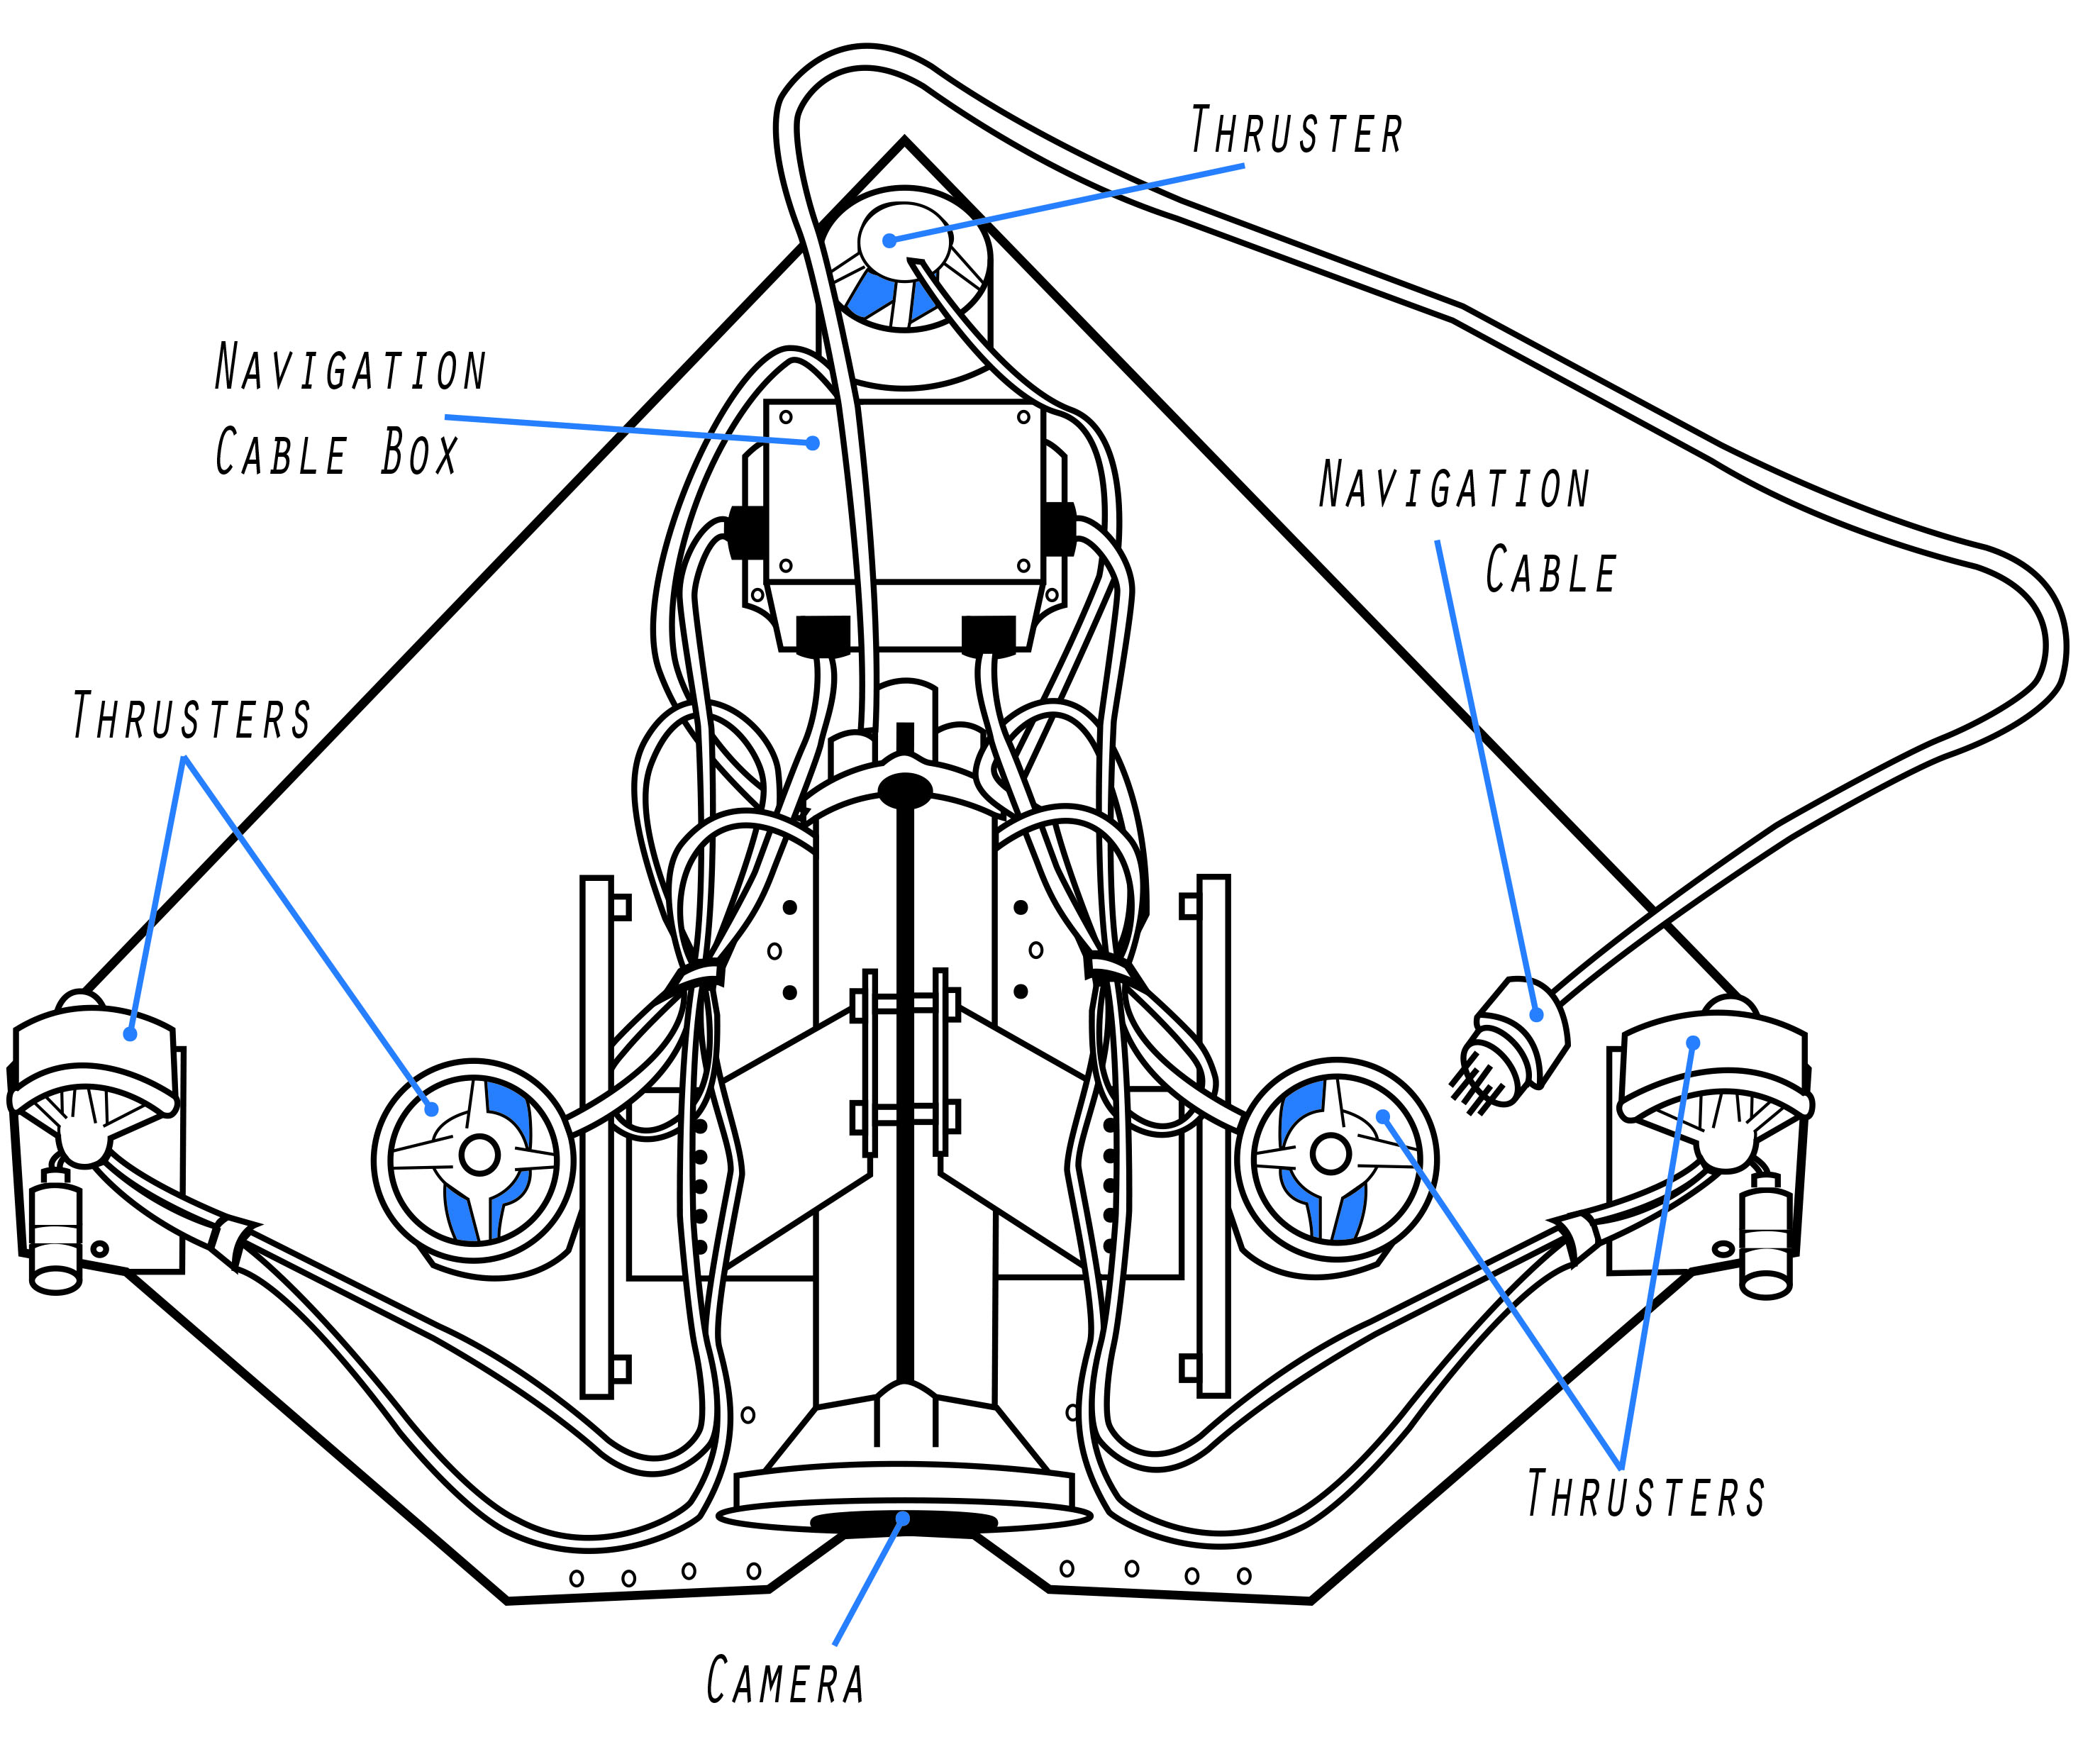
\includegraphics[width=1.4\columnwidth]{Figures/Component_Diagrams/inside_sub.jpg}
	\caption[]{An inside view of the submarine} % The text in the square bracket is the caption for the list of figures while the text in the curly brackets is the figure caption 
\end{figure}
\vspace*{5mm}
\begin{figure}[H]
	\centering 
	\hspace*{-2.5cm}
	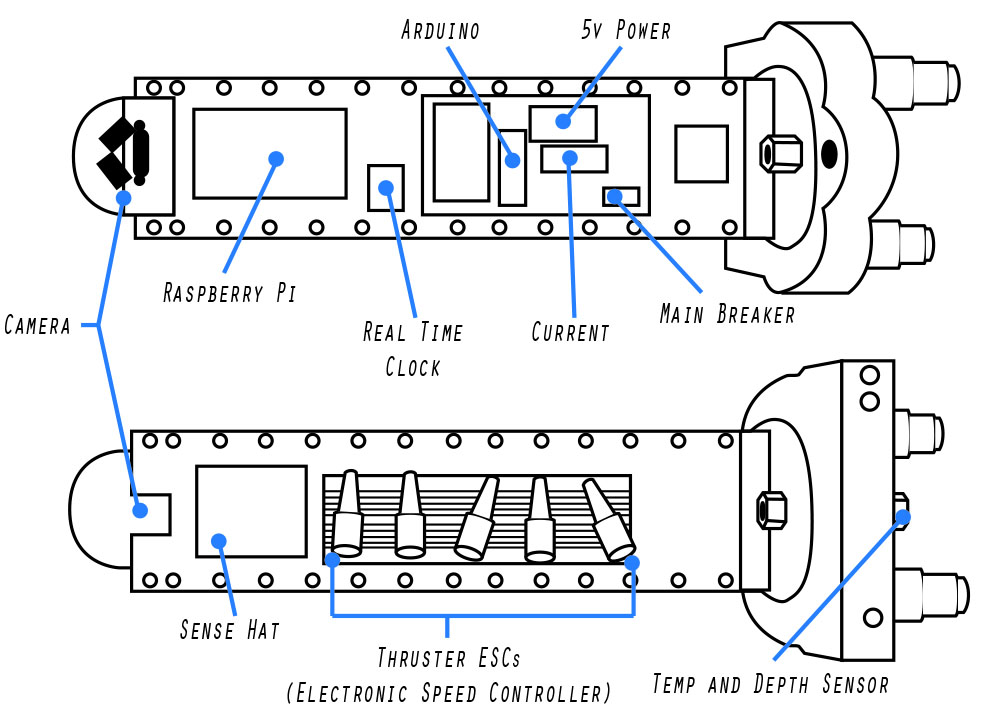
\includegraphics[width=1.4\columnwidth]{Figures/Component_Diagrams/navigation_board.jpg}
	\caption[]{An inside view of the submarines' camera main module} % The text in the square bracket is the caption for the list of figures while the text in the curly brackets is the figure caption 
\end{figure}
\vspace*{5mm}
\begin{figure}[H]
	\centering 
	\hspace*{-2.5cm}
	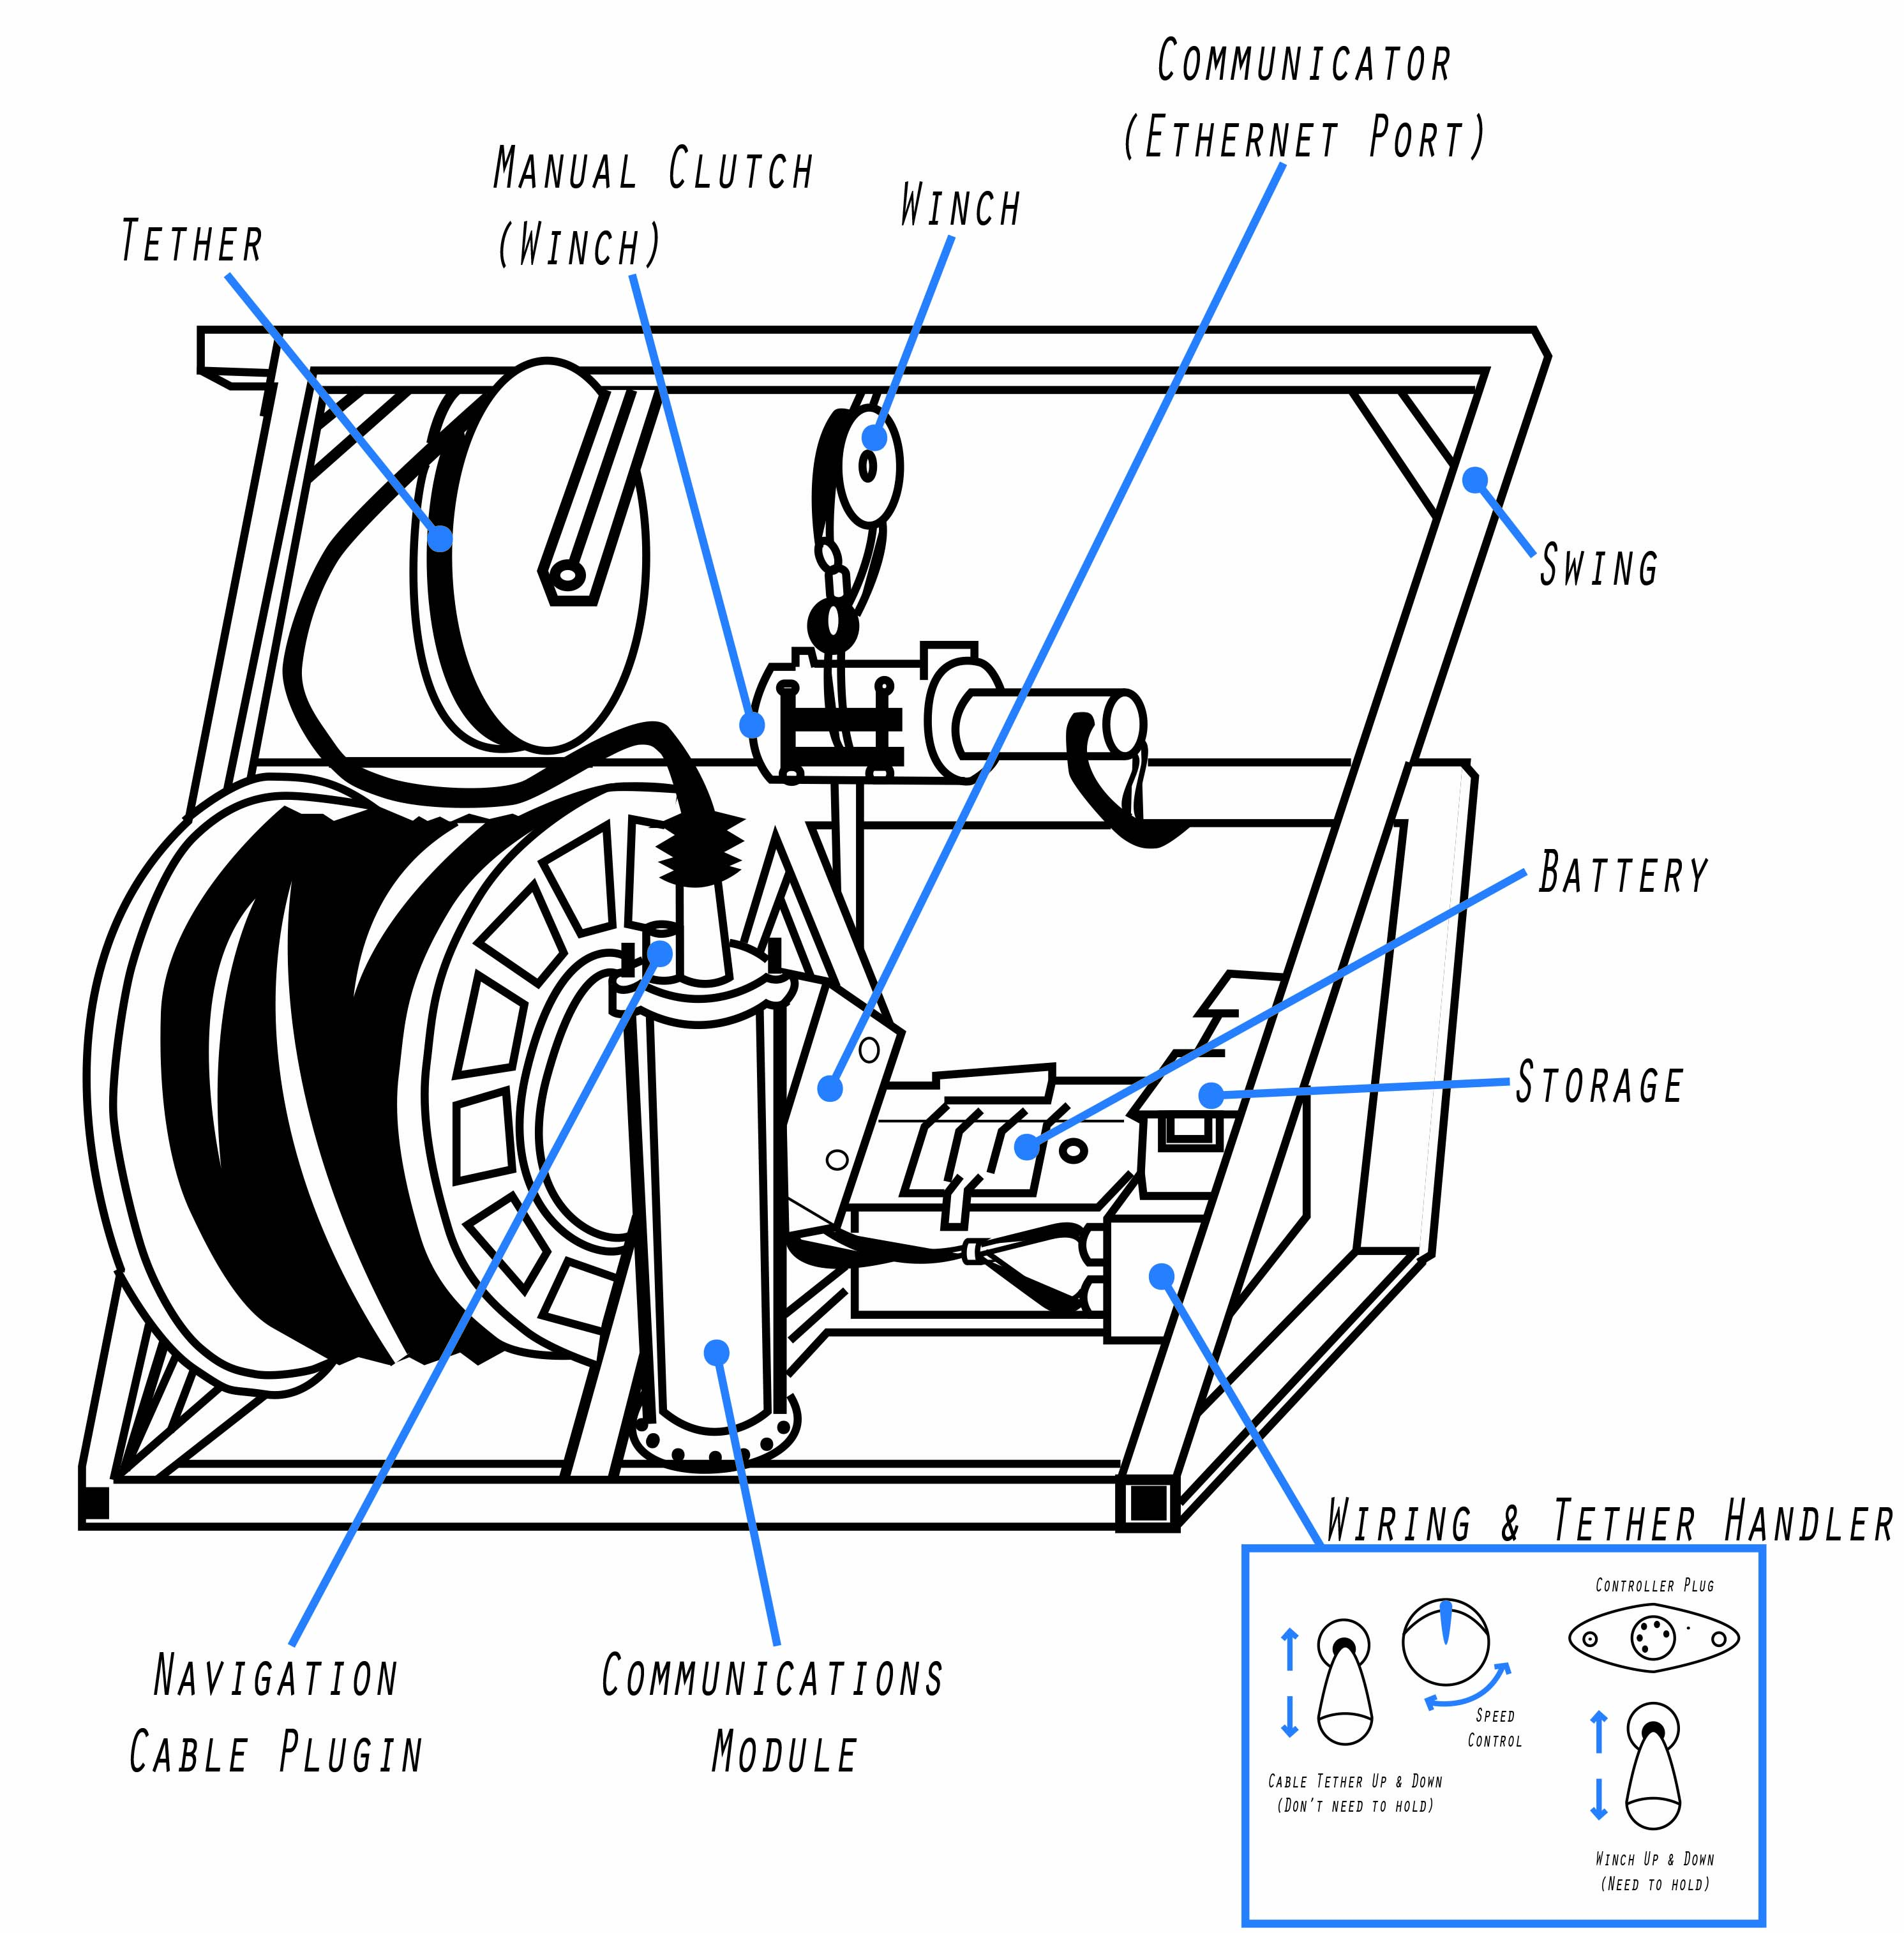
\includegraphics[width=1.4\columnwidth]{Figures/Component_Diagrams/handling_gear.jpg}
	\caption[]{An overview of the handling gear} % The text in the square bracket is the caption for the list of figures while the text in the curly brackets is the figure caption 
\end{figure}

%------------------------------------------------

\subsection{Schematics}

\begin{figure}[H]
	\centering 
	\hspace*{-2cm}
	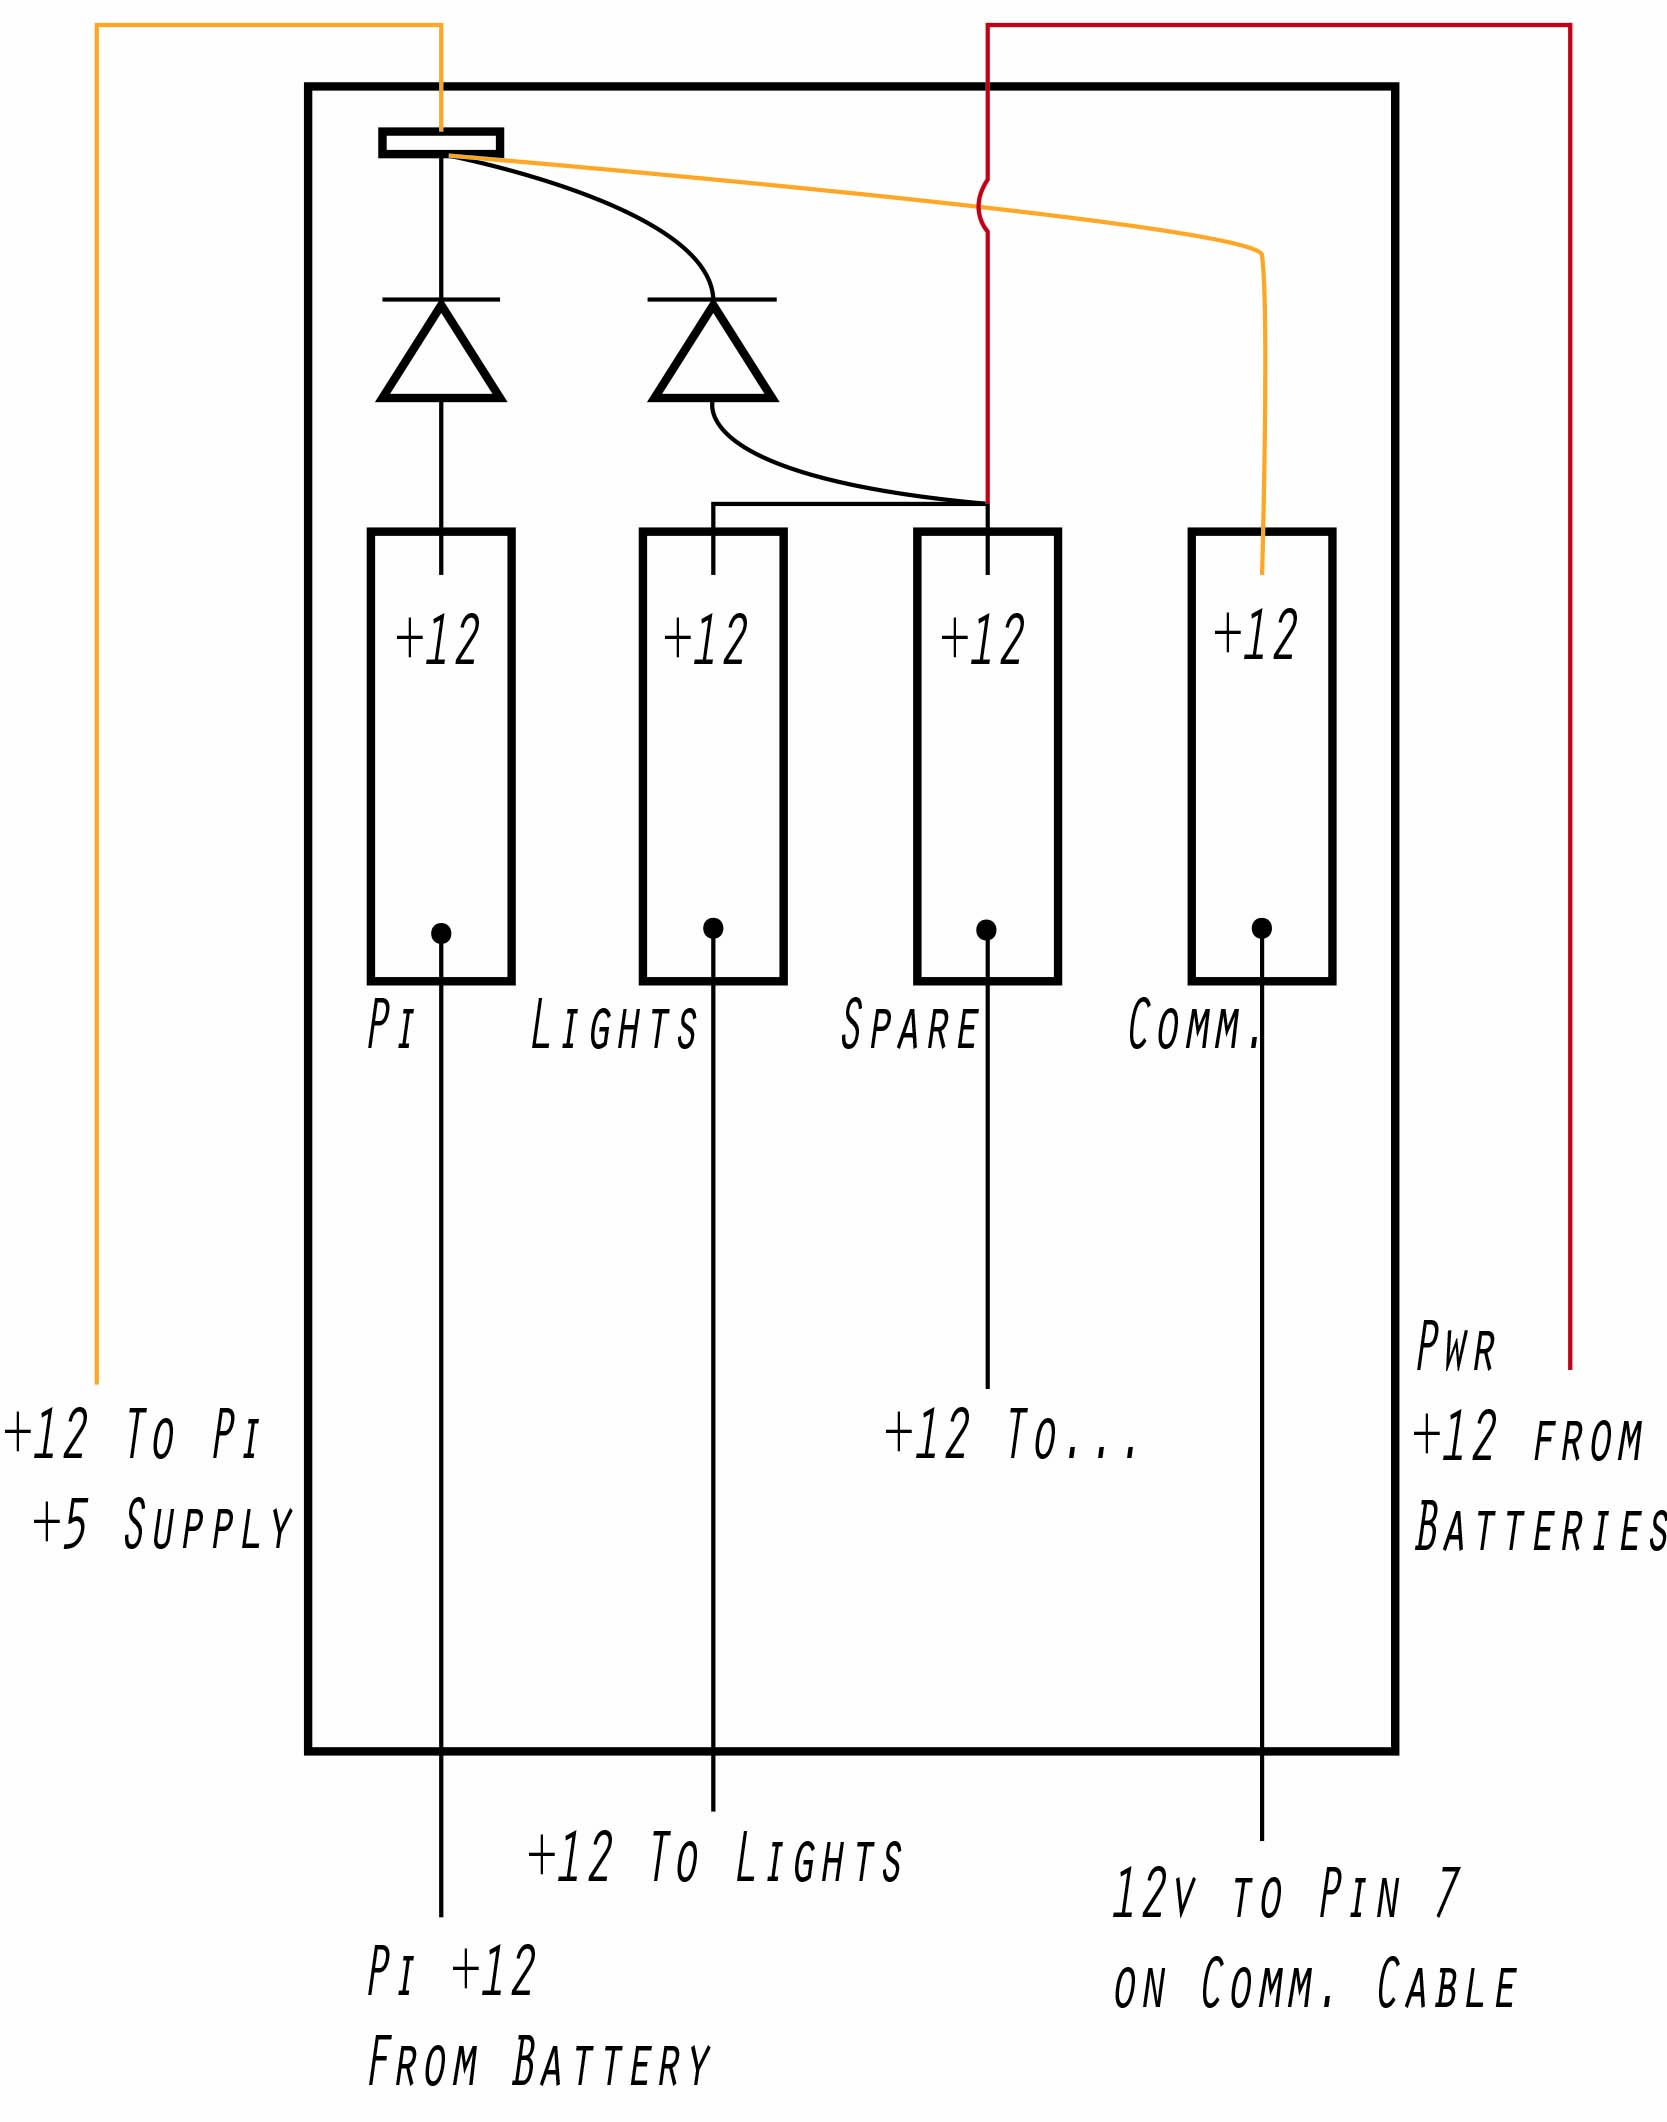
\includegraphics[width=1.1\columnwidth]{Figures/Component_Diagrams/fuse_schematic.jpg}
	\caption[]{Fuse Power Layout} % The text in the square bracket is the caption for the list of figures while the text in the curly brackets is the figure caption 
\end{figure}

\begin{figure}[H]
	\centering 
	\hspace*{-2cm}
	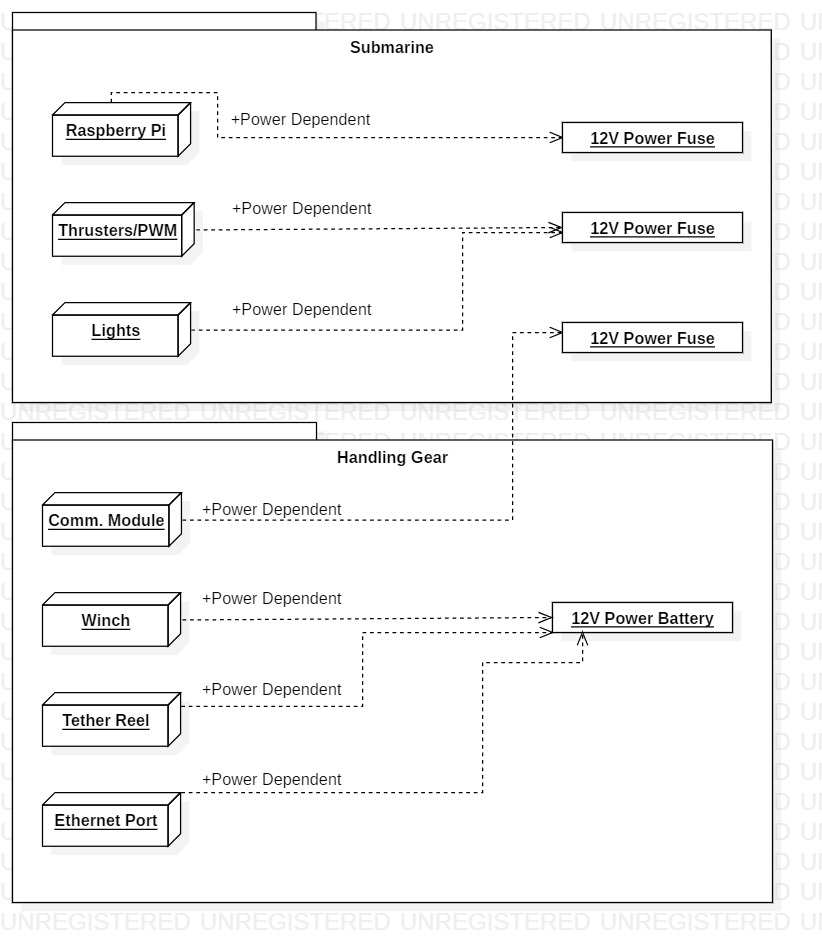
\includegraphics[width=1.1\columnwidth]{Figures/Component_Diagrams/schematic_pwr.jpg}
	\caption[]{Power Dependencies Layout} % The text in the square bracket is the caption for the list of figures while the text in the curly brackets is the figure caption 
\end{figure}

%------------------------------------------------

%------------------------------------------------

\subsection{Controller Layout}

\begin{figure}[H]
	\centering 
	\hspace*{-2.5cm}
	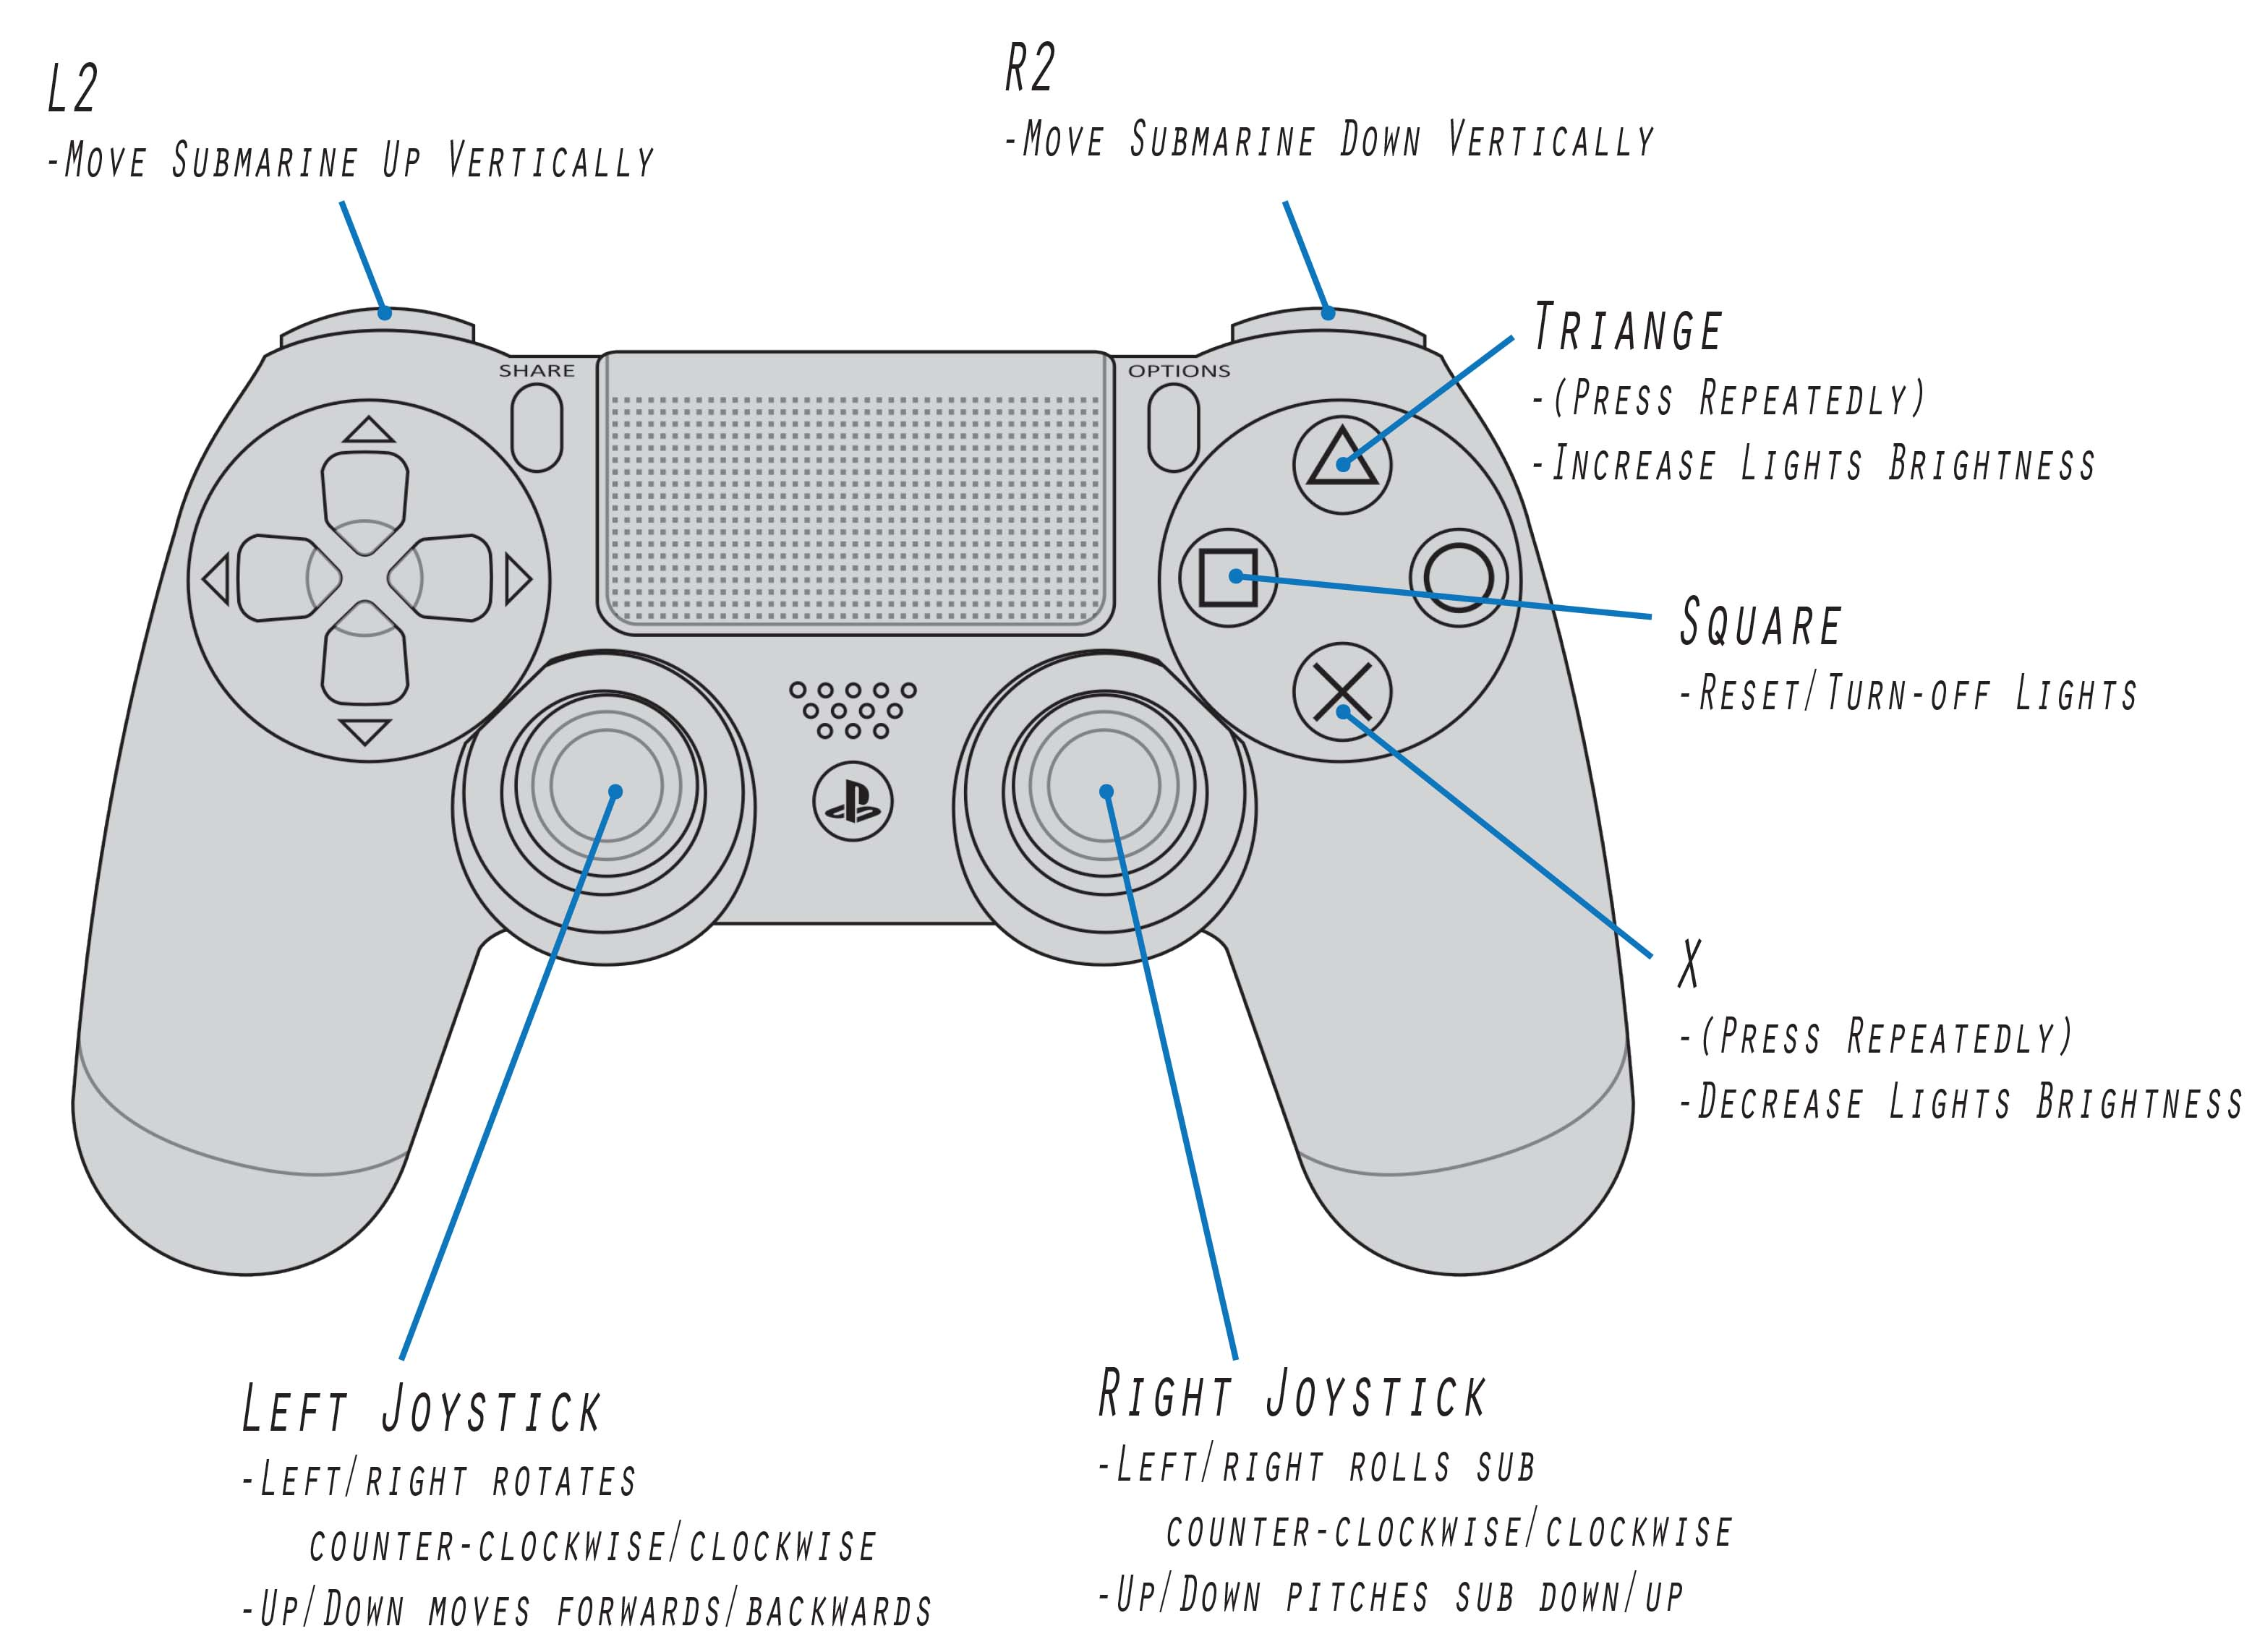
\includegraphics[width=1.4\columnwidth]{Figures/Component_Diagrams/dualshock_4_Layout.jpg}
	\caption[]{Current Controller Layout} % The text in the square bracket is the caption for the list of figures while the text in the curly brackets is the figure caption 
\end{figure}

\clearpage
\newpage
%------------------------------------------------

\subsection{Submarine Parts List}

The following is a list of components used inside the submarine:

\begin{itemize}
	\item Main Module
	\begin{itemize}
		\item Raspberry Pi 3
		\item 32 GB microSD card
		\item PiSense Hat (Internal pressure, temperature, compass, accelerometer, gyroscope)
		\item PWM Hat
		\item Realtime clock (pt. No DS1307)
		\item Arduino Nano for reading voltage
		\item ESC (x5)
		\item Power regulator
		\item Pressure/Temperature sensor for external treading
		\item Pi Camera V2
	\end{itemize}
	\item Communications Module
	\begin{itemize}
		\item Raspberry Pi 3
		\item 32GB microSD card
		\item External pressure/temperature sensor
		\item 1GB fiberoptic media converter
		\item 4-port GB switch
		\item Wide-angle camera
		\item Realtime clock (pt. No DS1307)
		\item Power supply
		\item An extra set of fiber connections for a second GB connection
	\end{itemize}
\end{itemize}

%------------------------------------------------

\subsection{Wiring Pins List}

The following is a list of the pins used per area. All wires are already numbered inside the submarines' main camera module. 

\begin{itemize}[noitemsep] % [noitemsep] removes whitespace between the items for a compact look
	\item Communications Module (12 Pins)
	\begin{itemize}[noitemsep]
		\item \#1 Ethernet Orange/White
		\item \#2 Ethernet Orange
		\item \#3 Ethernet Green/White
		\item \#4 Ethernet Green
		\item \#5 Ground
		\item \#6 Ground
		\item \#7 +12 VDC
		\item \#8-12 Unused
	\end{itemize}
	\item Main Module Tether (12 Pins)
		\begin{itemize}[noitemsep]
		\item \#1 Ethernet Orange/White
		\item \#2 Ethernet Orange
		\item \#3 Ethernet Green/White
		\item \#4 Ethernet Green
		\item \#5 Ground
		\item \#6 Ground
		\item \#7 +12 VDC
		\item \#8-12 Unused
	\end{itemize}
	\item Main Module Auxiliary (16 Pins)
		\begin{itemize}[noitemsep]
		\item \#1 Unused
		\item \#2 Unused +12 VDC
		\item \#3-16 Unused
	\end{itemize}
	\item Main Module Thrusters (16 Pins)
		\begin{itemize}[noitemsep]
		\item \#1-3 Left Horizontal Thruster
		\item \#4-6 Left Vertical Thruster
		\item \#7-9 Tail Vertical Thruster
		\item \#10-12 Right Vertical Thruster
		\item \#13-15 Right Horizontal Thruster
		\item \#16 Unused
	\end{itemize}
	\item Main Module Power (8 Pins)
		\begin{itemize}[noitemsep]
		\item \#1-4 Thruster Power
		\item \#5 CPU Power
		\item \#6-8 Thruster Power

	\end{itemize}
	\item Commutator (8 Contacts)
		\begin{itemize}[noitemsep]
		\item \#1-2 +9 VDC
		\item \#3-4 Ground
		\item \#5 Ethernet Green
		\item \#6 Ethernet Green/White
		\item \#7 Ethernet Orange
		\item \#8 Ethernet Orange/White
	\end{itemize}
	\item Onboard Power List
		\begin{itemize}[noitemsep]
		\item (3) 12V Lead Acid Batteries
		\item (2) +12 VDC to Thruster Power Switch
		\item (1) +12 VDC to CPU Power Switch
		\item (2) Ground to Frame
	\end{itemize}
	
\end{itemize}

%------------------------------------------------

\subsection{Power on/off}

Located on the back of the submarine is a power station with plugs. Each plug is labeled: PI, PWR, GRND. These are acronyms. PI stands for Raspberry Pi, it has its' own battery contained in the submarine. PWR runs to two separate batteries that have been linked together. Both batteries power the thrusters of the submarine. This is because the thrusters take so much power, by giving them two batteries, they last longer; also by separating them from the Raspberry Pi, if one dies it doesn't affect the integrity of the other. GRND stands for ground, its sole purpose is merely for charging the batteries.

%------------------------------------------------

\subsection{Charging Battery}

There are two separate chargers for charging the batteries as well as two separate sets of batteries. One set of batteries is inside the submarine, and the other set is on the handling gear.

\paragraph{The Charger}
The charger itself has an indicator on the back. By attaching the required charger to the battery it will tell you how much power is remaining as well as the charging progress. The charger also has a trickle feature, so it can be left plugged in overnight and will not overcharge the battery.\\ \\
There is also a charge indicator provided as a separate device. When measuring the charge, it is in voltage not percent. The nominal charge is 12V, fully charged is 13V, and low voltage is 11V. \\ \\
DO NOT let the batteries get below 11V. It is NOT recommended.

\paragraph{Submarine Battery Charge}
When charging the submarine, you can only charge one of the battery sets inside at a time. This is because of the way the charger was designed. So either the Raspberry Pi or the thrusters can be charged. \\ \\
In order to begin charging, the red attachment will be plugged into the desired battery port and the black attachment will always be plugged into ground. Charging the submarine (both battery sets) will take about 12 hours. It is recommended to charge the submarine after each deployment.

\paragraph{Handling Gear Charge}
When charging the handling gear, it functions in much the same way as the submarine. You will attach the charger to the handling gear battery, red to power and black to ground. Testing the handling gear battery charge is recommended but it lasts a very long period of time so frequent charges are not required.

%------------------------------------------------

\subsection{Dock Deployment}

The following section is the steps involved in an actual deployment of the Catfish while on a dock. In order to successfully place the submarine in the water, you will need both the submarine itself and its' handling gear. Once both are in position, act according to the following steps:

\begin{enumerate}
	\item Make the handling gear flat. This is done by removing the front wheel. All that needs to be done to accomplish this is to remove the bolt blocking the wheel from coming out and pulling on the wheel. The bolt itself can merely be pulled out by hand. If the wheel does not easily remove, a hammer may be needed to smack it out as it does get caught on the battery casing of the handling gear.
	\item Power on the handling gear. The switch is on the opposite side of the wiring \& tether handler.
	\item Next extend the swing to full height.
	\begin{itemize}
		\item First unhook the chains. You will need them to stabilize the handling gear swing as well as the pins.
		\item Then pull the handling gear swing upwards and outwards until it is fully extended. There are markers for convenience. You will need to make sure that both the winch line and the tether cable have enough slack to accomplish this. Directions for movement are on the components diagram for the handling gear as well as on the handling gear itself.
		\item After the swing is fully extended you will need to put the pins in the hole to block it and make sure it doesn't go back down. As you put the pins in make sure to pin the chains to the extended swing. This will make sure it doesn't fall flat and remains in the air at an angle.
		\begin{itemize}
			\item NOTE: The chains are uneven. The right chain will need to be two links in compared to the other chain. This evens it out more but one chain will still be more taut compared to the other.
		\end{itemize}
	\end{itemize}	
	\item Place the submarine in front of the handling gear. It is fine if it is at an angle because once linked to the winch it will straighten out. 
	\item Connect the submarine mast to the winch.
	\item Also connect the tether to the Communications Module. 
		\begin{itemize}
				\item NOTE: If there is power on, DO NOT let the pins of the communications module tether touch ANY metal. This will blow the fuse inside the submarine Main Module and there will be no ability for communication to the Catfish.
		\end{itemize}
	\item Then move the Communications Module to the slot on the mast, bolting it into place. Its camera will provide a top down view.
	\item Connect the ethernet cable from the host computer to the Communicator box. 
	\item Run through the software checks in the Checks section below.
	\item Power on the submarine by connecting both the PWM switch and the Pi switch located on the back of the submarine.		
	\item Before lifting the submarine, take out the bar from the top of the swing and place it in the slot at the bottom of the handling gear. The purpose of this is for one team member to stand on the bar, thus stabilizing the handling gear itself as the other team member lowers the submarine via the winch.
	\item Lift the submarine via the winch. 
	\item Lower the submarine into the water.
	\item After the submarine enters the water, reach over and pull the pin to release it from the winch. The tether will stay connected for now as it is our only connection to the submarine. It is also an emergency pull for the submarine.
		\begin{itemize}
				\item NOTE: If the submarine is lost/uncontrollable, it can be lifted via the tether. It is preferable to NOT pull it out of the water completely with the tether but it can be done.	
		\end{itemize}
	\item Control the submarine via controller or run the autonomous software (unavailable currently). 
\end{enumerate}

%------------------------------------------------

\subsection{Boat Deployment}

The following section is the steps involved in an actual deployment of the Catfish while on the LASES research boat. In order to successfully place the submarine in the water, you will need both the submarine itself and its' handling gear. Once both are in position, act according to the following steps:

\begin{enumerate}
	\item Make the handling gear flat. This is done by removing the front wheel. All that needs to be done to accomplish this is to remove the bolt blocking the wheel from coming out and pulling on the wheel. The bolt itself can merely be pulled out by hand. If the wheel does not easily remove, a hammer may be needed to smack it out as it does get caught on the battery casing of the handling gear.
	\item The handling gear should be against one side of the boat, in a position where it can extend towards the boat center.
	\item The submarine should be placed in front of the handling gear temporarily.
	\item Make sure the hoist is inserted into the metal slot closest to the boat cabin, opposite the handling gear.
	\item Power on the handling gear. The switch is on the opposite side of the wiring \& tether handler.
		\item Next pull the handling gear swing out.
	\begin{itemize}
		\item First unhook the chains from the pins on the handling gear. DO NOT remove the pins themselves, the handling gear does not need to extend fully.
		\item Then pull the handling gear swing outwards partially so that it is vertical. This is to prevent the tether wheel from grinding on the handling gear itself.
		\item After the swing is partially extended, reattach the chains.
	\end{itemize}	
	\item Extend the winch out to the hoist and put it through the small wheel located at the end of the hoist. The hoist itself acts as an extension of the handling gear.	
	\item Connect the tether to the Communications Module. 
	\begin{itemize}
		\item NOTE: If there is power on, DO NOT let the pins of the communications module tether touch ANY metal. This will blow the fuse inside the submarine Main Module and there will be no ability for communication to the Catfish.
	\end{itemize}
	\item Then move the Communications Module to the slot on the mast, bolting it into place. Its camera will provide a top down view.	
	\item Power on the submarine by connecting both the PWM switch and the Pi switch located on the back of the submarine.
	\item Connect the ethernet cable from the host computer to the Communicator box. 	
	\item Run through the software checks in the Checks section below.	
	\item Place the submarine on the side of the boat next to the hoist. The sub should be facing away from the hoist. (The Camera end is the front)	
	\item Attach the winch to the submarine at the base of the mast. (NOT the top for a boat dive) 
	\item Make sure one person is standing on the handling gear/bar. They will also be the one controlling the winch and the tether. (Refer to the components diagrams for controlling the winch and tether if needed)
	\item Lift the submarine.
	\item Push the submarine away from the boat and lower it.
	\item After the submarine enters the water, reach over and detach it from the winch. The tether will stay connected for now as it is our only connection to the submarine. It is also an emergency pull for the submarine.
	\begin{itemize}
		\item NOTE: If the submarine is lost/uncontrollable, it can be lifted via the tether. It is preferable to NOT pull it out of the water completely with the tether but it can be done.	
	\end{itemize}
	\item Control the submarine via controller or run the autonomous software (unavailable currently). 
		\begin{itemize}
		\item NOTE: At increased depths the submarine disconnects regularly. You may need to restart the thrusters.
		\item NOTE*: While using the submarine, make sure the tether stays away from the boat motor. Otherwise, it may cut the cable, thus losing the submarine.
	\end{itemize}
\end{enumerate}

%------------------------------------------------

\subsection{Catfish Collection}

When ready to collect the Catfish, use the following procedure:

\begin{enumerate}
	\item Using the controller or GPS location tracking (unavailable currently) to bring the submarine to the surface/find the submarine.
	\item If handling gear is not extended, refer to Deployment section for extending the handling gear. (Unless on a boat)
	\item Link the winch to the submarine mast. Operate winch to lift the submarine from the water.
		\begin{itemize}
			\item NOTE: Make sure to place the bar from the swing on the bottom of the handling gear and stand on it. You DON'T want to lose the handling gear.
		\end{itemize}
	\item Place submarine down. 
	\item Power off the submarine. This is done by detaching the top part of the power cables on the back.
	\item Unhook from winch and tether. Make sure to unbolt the Communications Module and replace on the handling gear.
		\begin{itemize}
			\item NOTE: DO NOT let the pins of the communications module tether touch ANY metal. This will blow the fuse inside the submarine Main Module and there will be no ability for communication to the Catfish.
		\end{itemize}
	\item Retract the handling gear. Unhook the pins and wrap the chains around the fully retracted swing. 
	\item Retract the winch wire and the tether.
	\item Power off the handling gear. The switch is on the opposite side of the winch \& tether control.
	\item Unhook the Ethernet cable from both connections. 
	\item Place cable and host laptop in bag. Place all tools in handling gear storage.
	\item Replace the wheel and bolt on the handling gear.
	\item Place the submarine and bag on the dolly.
\end{enumerate}

%------------------------------------------------

\subsection{Checks}

The purpose of these checks is to ensure the functionality of all submarine and handling gear parts both before and after deployment.

\paragraph{Handling Gear - Preoperational Checks} Before operating the handling gear, it is important to go through the following checks:

\begin{itemize}[noitemsep] % [noitemsep] removes whitespace between the items for a compact look
	\item Voltage check
	\item Winch check
	\item Reel check
	
\end{itemize}
Further descriptions of the aforementioned checks are as follows:

\begin{description}
	\item[Voltage Check] In order to check the voltage of the handling gear battery, merely use the provided voltage check device in the same manner as the battery charger.
	\begin{itemize}
		\item Attach the red wire to power and the black wire to ground.
	\end{itemize}  The handling gear battery is very long lasting and therefore this check does not need to be done after every deployment, but also should not be significantly deferred.
	\item[Winch Check] In order to make sure the winch wire itself isn't caught or in any way impeded, these short steps are needed:
	\begin{itemize}
		\item Merely release the manual winch switch and pull on the wire.
		\item Then, in order to rest the integrity of power raising/lowering of the wire, use the control box on the side of the handling gear.	
	\end{itemize}   Make sure to test both the forward and reverse aspects of the winch. 
	\item[Reel Check] The reel check is merely testing the large tether and making sure it has free movement and connection. The fiber-optic cable should be free to move, both in forward and reverse. There is a switch respective to this on the control box of the handling gear.
\end{description}

\paragraph{Submarine - Preoperational Checks} In order to ensure the integrity of the submarine hull prior to a deployment, the following checks should be conducted:

\begin{itemize}[noitemsep] % [noitemsep] removes whitespace between the items for a compact look
	\item Control module all thread torque checked
	\item Vertical thruster mount bolts checked
	\item Thruster to control module cables and connectors checked
	\item Light to control module cables and connectors checked
	\item Syntactic foam intact
	\item Other cables to control module?
	\item Mast attachment bolt torque checked
\end{itemize}

\paragraph{Software Checks} Prior to deployment of the submarine, the following software checks should be conducted:

\begin{itemize}[noitemsep] % [noitemsep] removes whitespace between the items for a compact look
	\item Ethernet cable connection to communications module box and host PC
	\item Ping from host PC terminal
	\item Open camera servers
	\item SSH into the submarine main Raspberry Pi
	\item Trusters check
\end{itemize}

\begin{description}
	\item[Pinging] 
	This check is to make sure that packets are being passed back and forth and that communication is happening.
	\item[Opening camera servers] 
	The camera servers are as follows:
	 
	\begin{itemize}[noitemsep]
		\item 192.168.2.1:8080/stream
		\item 192.168.2.2:8080/stream
	\end{itemize}

	If pictures or recordings are wanted, a separate program is needed.
	\item[Pi Login]
	The IP address of the Raspberry Pi in the submarine main module is 192.168.2.1. If you desire to access the Communications module Raspberry Pi is 192.168.2.2.
	\item[Trusters Check] When running python 3, file name thrusters\_client.py, output should give "connected to server". 
	\begin{itemize}
		\item If testing thruster function, barely push forward on a controller analog.
	\end{itemize} "Barely" is key because there is much less resistance in air than in water, so burning the thrusters is a risk.
\end{description}

\paragraph{Submarine - Postoperational Checks}

\begin{itemize}[noitemsep] % [noitemsep] removes whitespace between the items for a compact look
	\item Voltage check
	\item Physical check
	\item All shell bolts in-place and torque checked
	\item Vehicle to Communication module cable connected
	\item Final ballast system accessible
\end{itemize}

%------------------------------------------------

\subsection{Getting Inside the Catfish}

The Catfish itself is not watertight. It is divided into two halves, the upper and lower parts. The upper part of the submarine contains all the electronics, thrusters, and wires. The lower part of the submarine has the ballast and buoyancy materials. Water flows freely through all parts except the Main Module. The wires inside the Navigation Cable Box are waterproofed as well. If for any reason the inside of the Catfish needs to be accessed, please refer to the following sections: 

\paragraph{Removing the Hull} This is fairly simple, all that is needed is to remove the screws. 

\begin{enumerate}
	\item First, all the screws and bolts around the outside of the submarine EXCEPT the thruster screws/bolts will be removed. The reason for this is that it is easier to manage the thrusters falling off when they are the last to be removed. 
	\item Next you remove the mast bolt and the mast itself. Once this is done, the top hull can be removed from the submarine. \\
\end{enumerate}
	If you want to access the Main Module, then follow the next directions. 
\begin{enumerate}
	\item First you want to unscrew the 2 6mm bolts under the face of the submarine camera. 
	\item You also need to remove the bolts and washers from the long metal rods around the Main Module. 
	\item Then you can slide the assembly off the insides of the module.
\end{enumerate}

 Refer to diagram above in the Components section for an outline of the module.
 
\paragraph{Reattaching the Hull} When ready to reattach the Main Module and hull, please follow these directions. \\

First is the reassembly of the Main Module casing.
\begin{enumerate}
	\item  Make sure all the ends are clean, both on the metal rods and the cylinder casing. 
	\item Also make sure the O-Rings are clean. Grease both ends of the cylindrical casing with silicon grease, a little grease goes a long way. This process is just to make the O-Rings happier when under pressure. 
	\item Then you will slide this assembly back onto the Main Module insides, tucking in the wires as you go and pushing it taut. 
	\item While keeping pressure up put the washers and bolts back in place on the long metal rods, these should spin on easily. If they do not, then you are using the bolts for the outside of the hull and not the ones for the Main Module. 
	\item Lastly, screw in the 2 6mm bolts back under the face of the submarine camera. This can be done by hand. In order to test the tightness of the Main Module, you can use sound. Merely pull the rods like a guitar string and make sure they all sound the same. The face of the camera should be flush with the submarine.\\
\end{enumerate}

Next is the hull of the submarine.

\begin{enumerate}
	\item To reattach the hull itself, just place the hull in place and screw in all the bolts except the thrusters and lights. 
	\item After all the screws/bolts are in place, reattach the thrusters and then the lights which go under the thrusters. The lights can be pointed in different directions using the screw on the mount. 
	\item After everything is tight, the mast can be reattached. The submarine is now reassembled.
\end{enumerate}

%------------------------------------------------

%----------------------------------------------------------------------------------------
%	USING SOFTWARE
%----------------------------------------------------------------------------------------

\section{Using Software}
%------------------------------------------------

\subsection{Connecting to the Submarine}
In order to connect to the Submarine Raspberry Pi, depending on which type of connection that is to be used, refer to one of the following sections:

\paragraph{Ethernet Connection}
\begin{enumerate}
	\item First, connect the Ethernet cord to the Communications box and connect the Navigation Cable to the Communications Module.	
	\item Make sure everything is turned on. (Hangling Gear, Submarine) 
	\item Next you can either VNC or SSH into the Raspberry Pi. The IP for this will be 192.168.2.1.
	\begin{itemize}
		\item Default Username: pi
		\item Defualt Password: makerspace
	\end{itemize}
	\item Then open thruster\_client.py and change the host IP value to 192.168.2.1 (This will differ if using a new submarine as this static Ethernet IP is one we have configured.)
	\item You can then refer to the section "Software Checks" for specifics on checking the connection.
\end{enumerate}

\paragraph{Wireless Connection}
\begin{enumerate}
	\item You will not need an wired connection at all to the submarine to access this way. This cannot be done underwater.	
	\item Make sure everything is turned on. (Submarine) 
	\item Next you can either VNC or SSH into the Raspberry Pi. The IP for this will be 192.168.0.207.
	\begin{itemize}
		\item Default Username: pi
		\item Defualt Password: makerspace
	\end{itemize}
	\item Then go to thruster\_client.py and change the host IP value to 192.168.0.207 (This will differ if using a new submarine as this static Wireless IP is one we have configured.)
	\item You can then refer to the section "Software Checks" for specifics on checking the connection.
\end{enumerate}

%------------------------------------------------
%------------------------------------------------

\subsection{Acquiring the Code}
In order to run or change anything, you need to have the code first. The following sections relate to either obtaining the code, or installing various programs needed to make it run.

\paragraph{GitKraken}
One of the first things you'll want is something called GitKraken. It's a program that interfaces with Github in a way that makes it easier to pull, push, and commit changes. It will also automatically store any updates from any pulls in a local file designated by you. 

Its' ability to sync up to Github and show any forks or files that others are working on is great.If you link to any additional repositories, it will also keep track of those for you.

\paragraph{Python 3}
You will need python 3 as all the code is written using it. Python 2.7 won't work, it has to be 3. In order to check this, just run the command "python3" in a terminal window. If it is not there, you will need to install it based on your OS' directions.

\paragraph{Pygame - Python 3 version}
This install also differs based on OS. It will correspond with the Python 3 version. The purpose of pygame is to keep track of the controller so if you plan on using it you will need this program.

\paragraph{Cloning the Repository}
By using Gitkraken, you can just clone the repository directly into your file system. Afterwards you will need to also acquiesce to the request that Gitkraken makes to pull files relating to the linking of the CDA Catfish repository and Gizmo's original code repository.

\paragraph{Making a Path}
	\begin{itemize}
		\item In order to make a shortcut path for when you're typing in the 'thruster\_client.py' command, you will need to edit your 'bash.rc'.
		\item Then you will need to input the following line:
		
		"alias g2x\_c = "PATH\_STRING\_HERE""
		\item This will make it so you can just type 'cd g2x\_c' to move straight to the folder where 'thruster\_client.py' is.
	\end{itemize} 

 While this section isn't needed, it makes life a bit easier.
%------------------------------------------------
%------------------------------------------------

\subsection{Moving the Submarine}



%------------------------------------------------
%------------------------------------------------

\subsection{Running in Simulation Mode}
For the purpose of testing the submarine movement or code while NOT burning out the thrusters, it's important to place the submarine thrusters into simulation mode. This will simulate the thruster movement without the danger of burning out the thrusters. It is especially important because air has less resistance than water, which the thrusters are built for a water environment.

\begin{enumerate}
	\item SSH into the submarines' Raspberry Pi (or VNC)
	\item Run the command 'sudo systemctl stop g2x-thruster.service'
	\item Run the command 'g2x\_c' (if you have set up the path shortcut mentioned in the section "Making a Path"). If not the path is as follows: '~/Documents/Projects/g2x-submarine-v2/services/controllers'
	\item Run the command './thruster-server.py -s -v' . This command simulates the thruster response.
\end{enumerate}



%------------------------------------------------

%------------------------------------------------

\subsection{Taking Pics/Video}
When connecting to the stream servers, you are then able to record video or take screenshots. However, in order to accomplish this you need seperate software to record your screen. We are using the XBOX Apps' recording tools on Windows. This can be accessed by pushing the Windows Button and the 'G' key at the same time.

\paragraph{Where to Save} 
If using the XBOX App then all videos and screenshots will save to the Capture folder in the Videos folder. In order to move this, you just have to move the folder.

\paragraph{Streaming} 
The XBOX App also has a streaming feature that we have yet to experiment with.

%------------------------------------------------

%----------------------------------------------------------------------------------------
%	SYSTEM CONFIG
%----------------------------------------------------------------------------------------

\section{System Configuration}



%------------------------------------------------

\subsection{Configuring 3D map?}


\subsubsection{Testing with the Turtle}


\subsubsection{Mapping Underwater}


%------------------------------------------------

--------------------------------
%	CONSUMER INFO
%----------------------------------------------------------------------------------------

\section{Consumer Info}

\subsection{Troubleshooting}

\paragraph{Known Ubuntu Issues}
\begin{itemize}
	\item THRUSTERS OUT OF CONTROL
	
	When the controller isn't plugged in, Ubuntu thinks it is still receiving input from it. Thus, the thrusters will go haywire and will need to be unplugged. 
	
	Could be a kernel issue, or just an Ubuntu issue, still unsure.
	
	Right now we know that Ubuntu automatically connects to and receives input from the onboard laptop accellerometer. When connecting a controller, it also recieves both the input from the PS4 controller AND its gyroscope as seperate inputs. 
	
	Thus when running 'thruster\_client.py', it is receiving all three of these inputs and thus the thrusters go crazy.
	
	We have inputed a fix into the code that checks the name of the joystick. If the controller is not plugged in, it exits. If it is plugged in, it matches the name and ONLY the input from the controller itself is taken.
	
	NOTE 6/27/2018 Thrusters still go crazy
	
	Currently in order to resolve this, we are only running the software on either a Windows or a Mac machine. Our Ubuntu laptop is only being used for mapping purposes.
	
\end{itemize}

\begin{itemize}
	\item BUTTONS ARE WEIRD BETWEEN UBUNTU AND OTHER OS. 
	
	Kernel problems. Light buttons are mixed up. Square is bright, X is reset, O is dim.
\end{itemize}

\begin{itemize}
	\item LIGHTS WONT COME ON. 
	
	Just hit the Square button then Triange again. The lights should come on.
\end{itemize}

\begin{itemize}
	\item PYGAME MODULE ISN'T FOUND/DOESN'T EXIST. 
	
	There is a super long fix for this that involves multiple installs, upgrades, and updates. If we get around to documenting, it will go here.
\end{itemize}


\end{document}